\documentclass[dvipsnames]{article}
\usepackage[ff,sets,adversary,advantage,keys,primitives,operators,lambda,logic,notions]{cryptocode}
\usepackage{boxedminipage}
\usepackage{comment}
\usepackage[utf8x]{inputenc}
\usepackage{subcaption} % for double figures
\usepackage{bm} % for bold math symbols
\usepackage{float}
\usepackage{color}
\usepackage{xcolor}
\usepackage{xspace}
\usepackage{url}
\usepackage{tabularx}
\usepackage{booktabs}
\usepackage[capitalise]{cleveref}
\usepackage{enumitem} % used to reduce indent of {itemize}

\colorlet{party}{Brown}
\colorlet{randomness}{Maroon}
\colorlet{protocol}{Black}
\colorlet{string}{BlueViolet}
\colorlet{entry}{NavyBlue}
\colorlet{public}{OliveGreen}
\colorlet{private}{Plum}

% comments
\newcommand{\fanz}[1]{\textsf{\color{red}{[[Fan: #1]]}}}


% protocol boxes
\newcommand{\stringlitt}[1]{\textcolor{string}{\text{``#1''}}}
\newcommand{\msgok}{\stringlitt{ok}}
\newcommand{\msgsched}{\stringlitt{sched}}
\newcommand{\msgproof}{\stringlitt{proof}}
\newcommand{\msgack}{\stringlitt{ack}}
\newcommand{\msgfinP}{\stringlitt{proverFinished}}
\newcommand{\msgfinS}{\stringlitt{serverFinished}}
\newcommand{\timeout}{\ensuremath{\mathsf{timeout}}}

\newcommand{\onrecv}{\textcolor{entry}{\bf On receiving}\xspace}
\newcommand{\oninit}{\textcolor{entry}{\bf On initialization}\xspace}

\renewcommand{\pccomment}[1]{\text{\textcolor{gray}{\scriptsize // #1}}}
\newcommand{\protocol}[3][\columnwidth]{
  \begin{boxedminipage}[t]{#1}
    \begin{center}\textbf{#2}\end{center}

    \procedure[mode=text, codesize=\small]{}{
      #3
    }
  \end{boxedminipage}
}

\newcommand{\etal}{\textit{et al.}\xspace}

\newcommand{\enclavekey}{\pk_{\text{TEE}}}
\newcommand{\signed}[2]{\ensuremath{\langle{#1}\rangle_{#2}}}
\newcommand{\aux}{\mathsf{aux}}
\newcommand{\ticket}{\mathcal{T}}
\newcommand{\usermessage}{\mathcal{M}}

\title{Trustless Hardware and its Applications in Dinning Cryptographers}
\author{censored}
\begin{document}
\maketitle

\section{Introduction}

\section{Protocol Overview}

\paragraph{Notation.} We use $\signed{m}{\pk}$ to denote a message signed by the secret key of $\pk$.

\paragraph{Overview.}

There are three types of players:

\begin{itemize}
    \item Any trust servers $(S_1, \dots, S_\ell)$ running~\cref{proto:server}.
    \item Aggregators (each with an SGX enclave) $(A_1, \dots, A_m)$ running~\cref{proto:agg}.
    \item Users (each with an SGX enclave) $(U_1, \dots, U_n)$ running~\cref{proto:user}.
\end{itemize}

\begin{figure}
\protocol{Protocol of a user $U_i$ (and her enclave)}{
\textbf{State:} \\
\begin{itemize}[leftmargin=*]
    \item $(\sk, \pk)$ a pair of keys generated in an enclave. $\pk$ is published in an attestation. $\sk$ is sealed to persistent storage for backup.
    \item Pair-wise keys with all servers: $K_{i,j} \in \bin^\secpar$ for $j\in [\ell]$.
\end{itemize}
\textbf{Registration:} \\
\t $U_i$ talks to all servers to generate keys and store them. $U_i$ also registers the public key of her local enclave $\enclavekey$. \\[2mm]
\textbf{Scheduling:}\fanz{changed to be specific to footprint scheduling. How to enable multiple people speak in the same round.} \\
\underline{Enclave:} User's scheduling enclave has the following function.\\
\t def $schedule(m, T) \to ({\sf State}, T')$: \fanz{how to authenticate $m$?}\\
\t\t \pcif $T=\bot$ \pcthen \\
\t\t\t \pccomment{start by trying to schedule all $S$ slots. $m_\text{out}$ contains footprints} \\
\t\t\t \pcreturn $({\sf Continue}, (1, \set{1,\cdots,S}, m_\text{out})$ \\
\t\t assert $m\neq \bot$. Parse $T$ as $(i, \mathcal{S}, m_\text{out})$. \\
\t\t \pcif $i = R-1$, \pcthen \pcreturn $({\sf Done}, T_\text{final}={\sf Finalize}(m,T)$) \pccomment{Finalize the final result} \\
\t\t $T' \gets \mathsf{TrySchedule}(i,m,\mathcal{S})$ \pccomment{determines if it continues to schedule for this cycle. If not, $T'=\bot$. Otherwise, it computes $\mathcal{S}'$---slots to reserve next, as well as new footprint message $m'$, and return $T'=(i+1, \mathcal{S}', m')$} \\
\t\t \pcif $T'=\bot$ \pcthen \pcreturn $({\sf Abort}, \bot)$. \\
\t\t \pcelse \pcreturn $({\sf Continue}, T'$) \\[2mm]
%
\underline{User:} $U_i$ calls $(s, T)\gets schedule(\bot,\bot)$ (in her scheduling enclave) to initialize the scheduling protocol. The enclave returns a state $s$ and a ticket $T$. If $s = {\sf Continue}$, user parses $T$ as $(\_,\_, m)$ and sends $m$ in the next round. User keeps doing so until $s={\sf Done}$ (or abort where user just aborts) and use $T$ as the final ticket $\ticket=\signed{{r_1, r_2, \cdots, r_k}}{\enclavekey}$ where $\set{r_i}_i$ are rounds reserved for $U_i$. \\[2mm]
\textbf{Submission:} \\
\fanz{old text. need to be made compatible with footprint scheduling}
$U_i$ sends $(\ticket, m)$ to her enclave where $m$ is the message. The enclave verifies the ticket and forms a broadcast message $M_i$ containing $m$ in slots $(s_l,s_h)$, and zeroes otherwise. The enclave then computes pads (stretch the key as needed) $K_{i}=\oplus_{j=1}^{\ell} \prg(K_{i,j}\|r)$ and outputs $\usermessage_i=\signed{U_i, c_i=M_i \xor K_i}{\pk}$. $U_i$ submits $\usermessage$ to one or more of the aggregators. \\[2mm]
\textbf{Output:} \\
Wait to receive the final outcome from aggregators $(r, \vec{m}, \vec{\sigma})$.
}
\caption{User protocol}
\label{proto:user}
\end{figure}

\begin{figure}
\protocol{Protocol of an aggregator $A$ (and her enclave)}{
\textbf{State:} \\
\begin{itemize}[leftmargin=*]
    \item $(\sk_A, \pk_A)$: key pair. Ditto.
    \item A mapping $(r, \mathcal{U}, c)$ storing the aggregated messages so far (for round $r$).
\end{itemize}
\textbf{Aggregate}($U_i, c_i$): \\
\t Retrieve $(r, \mathcal{U}, c)$ from local storage. If $U_i\in\mathcal{U}$, ignore and return. If not, store $(r, U_i, c_i)$ for reasons that will become clear shortly, set $\mathcal{U}:=\set{U_i} \cup \mathcal{U}$ and $c:=c_i \xor c$. Broadcast $(r,\mathcal{U}, c)$ to other aggregators. When $|\cal U|$ is big enough or a timeout has passed, $A$ sends $(r,\mathcal{U}, c)$ to all servers. \\
\textbf{Catchup}: \\
\t When receiving $(r,\mathcal{U}', c')$ from a peer aggregator $A'$, catch up if needed. \fanz{$A$ can't simply xor with $c'$ if $U$ overlaps with $U'$. But it's not hard either given both are honest.} \\
\textbf{Finalize:} \\
\t After receiving signed pads $(r, K_{S_j}, L_r)$ from all servers, $A$ computes $m=c_r \xor K_{S_1} \xor K_{S_2} \dots \xor K_{S_\ell}$, signs it, and sends to all connected clients. Proceed to round $r+1$.
}
\caption{aggregator protocol\fanz{enclave is stateless. state is stored out of aggregator.}}
\label{proto:agg}
\end{figure}

\begin{figure}
\protocol{Protocol of a server $S_i$\fanz{no need for SGX unless for defense-in-depth?}}{
\textbf{Finalize:} \\
\begin{itemize}[leftmargin=*]
\item Upon receiving from all aggregators or the round closure deadline has passed, the server $S_j$ forms a list $L_j$ of all client identifiers included in aggregator messages. Broadcast $L_j$ to other servers.
\item Given all servers' lists, the servers determines a list $L_r$ of clients who submitted in round $r$. Talking to the aggregator if needed (e.g., to retrieve messages not aggregated), all servers reach agreement on the final aggregated message $c_r = \bigoplus_{i \in L_r} c_i$.\fanz{alternatively, we could have aggregators to reach consensus first, and servers just take the largest aggregation set as $L_r$.}
\item Each server $S_j$ computes her pad $K_{S_j}=\bigoplus_{i\in L_r}{K_{i,j}}$ and broadcast $\signed{r, K_{S_j}, L_r}{\pk_{S_j}}$ to connected aggregators.\fanz{in Dissent this is sent to the clients directly but in our setting the server doesn't interact with clients directly.}
\end{itemize}
}
\caption{server protocol}
\label{proto:server}
\end{figure}

\subsection{Footprint scheduling}

We use footprint scheduling to assign participants to rounds, so that ideally
only one participant sends messages in a given round.

The ideal functionality of scheduling takes as input a list $\mathcal{U}$ of users who wish to speak in the next $S$ rounds, outputs a list of $S$ identities $(U_1, U_2, \dots, U_S)$ such that $U_i \in \mathcal{U}$,
which schedules $U_i$ to speak at the $i$th round.\fanz{how do we allow multiple people to speak in the same round?}
Note that if $|\mathcal{U}|<S$, the output may contain duplicated identities.

Footprint scheduling is done $R=\log(N)$ rounds. When $R \le S$, scheduling rounds can be piggyback on normal message, like in~\cref{fig:message}.

\begin{figure}[H]
    % \includegraphics[page=6,width=\columnwidth]{all-images.pdf}
    \centering
    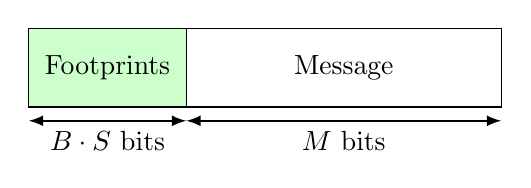
\begin{tikzpicture}[
    scheduling/.style={draw=black, fill=green!20},
    bigbrace/.style={decorate,decoration={brace,amplitude=5pt,raise=4pt}},
    bigbracemirror/.style={decorate,decoration={brace,mirror,amplitude=5pt,raise=4pt}},
    ]
    \draw[scheduling] (0, 0) rectangle (2, 1);
    \draw (2, 0) rectangle (6,1);
    \draw (1, .5) node[align=center] {Footprints} +(3, 0) node {Message};
    \draw[<->, thick, >=latex, yshift=-5pt] (0.0, 0) -- (2, 0) node [black,midway,below] {$B\cdot S$ bits};
    \draw[<->, thick, >=latex, yshift=-5pt] (2, 0) -- (6, 0) node [black,midway,below] {$M$ bits};
    \end{tikzpicture}
    \caption{A DC net message consisting of a footprints for scheduling  (green part; up to $B\cdot S$ bits) and regular message}
    \label{fig:message}
    \end{figure}



\end{document}